%Vorlage fuer Thesen an der FFHS
\documentclass{ffhsthesis}

\usepackage[utf8]{inputenc}
\usepackage[ngerman]{babel}
\usepackage[autostyle=true,german=quotes]{csquotes}
\usepackage[labelformat=simple]{caption}
\usepackage{siunitx}
\usepackage{amssymb}
\usepackage{tikz}
\usepackage{booktabs}
\usepackage{minted}
\usepackage{float}
\usetikzlibrary{positioning, matrix, shadows, shapes.multipart}
\renewcommand{\figurename}{Abb.}

\begin{document}

\dokumentTyp{Disposition zur Seminararbeit}
\studiengang{INF}
\title{Vergleich von Graph-Kompressionsalgorithmen $k^{2}$ Tree und Huffman Encoding zur Komprimierung von Barabási-Albert Graphen}
\subtitle{Seminararbeit} % optional
\titelbild[width=8cm]{logo.png}  % optional
\author{Matthias Heimberg}
% \date{}
\wohnort{Melchnau}
%\referent{Name des Referenten\\ Titel\\Unterrichtetes Fach}
\referentin{Usrula Deriu\\ Dozentin\\SemA INF}
\eingereichtBei{Usrula Deriu\\ Dozentin\\SemA INF} 


\maketitle
\chapter*{Zusammenfassung}
In der Arbeit wurden die beiden Kompressionsalgorithmen K2-Tree und Huffman Encoding zur verlustfreien Kompression auf Barabási-Albert Graphen angewandt. Die Kompressionsalgorithmen wurden bezüglich Kompressionsfaktor und Kompressionszeit verglichen. Beide Algorithmen wurden auf Basis der Literaturdaten eigenständig in Python implementiert. 

Die erzielten Ergebnisse zeigen deutlich, dass der Huffman Algorithmus den Algorithmus $k^2$-Tree hinsichtlich der Kompressionszeit und des Kompressionsfaktors übertrifft. Als Faktoren, welche die Leistung der Algorithmen beeinflussen wurden primär die Graphengrösse und die Graphendichte identifiziert. Diese Erkenntnisse können zur Optimierung der Kompressionsstrategie genutzt werden und bieten einen Ausgangspunkt für zukünftige Forschungen zur Graphenkompression.

\tableofcontents


\startThesis % Befehl muss vor dem ersten chapter stehen (Seitennummerierung!)



\chapter{Einleitung} 

Die digitale Revolution hat zu einer exponentiellen Zunahme von Daten geführt, die in Form von Graphen repräsentiert werden können. Graphen stellen komplexe Beziehungen und Muster dar und finden heute Anwendung in den unterschiedlichsten Disziplinen, wie in den Sozialwissenschaften, in der Netzwerkanalyse und in der Bioinformatik. Angesichts der wachsenden Grösse und Komplexität von Graphen sind effiziente Speicher- und Verarbeitungsstrategien von grosser Bedeutung. Eine der Strategien ist die Datenkompression, die den Speicherplatz und die Verarbeitungszeit für die Handhabung von Graphen reduziert.

In dieser Arbeit wird die Kompression von Graphen untersucht. Insbesondere wird die Effizienz und Wirksamkeit zweier Kompressionsalgorithmen, K2-Tree und Huffman Encoding im Kontext von Barabási-Albert Graphen, einem gängigen Modell für komplexe Netzwerke, evaluiert und verglichen.

\section{Motivation}
In einer Zeit in welcher das Volumen, die Vielfalt und die Geschwindigkeit der Datenerzeugung exponentiell zunimmt \cite{naeem2022trends}, ist die effiziente Speicherung und Verarbeitung von Daten zu einer grossen Herausforderung geworden. Graphen repräsentieren komplexe Strukturen und Beziehungen in solchen Datensätzen und haben dadurch in unterschiedlichen Disziplinen eine zentrale Rolle eingenommen. Um mit Graphen von grossen Datensätzen umgehen zu können, wurden unterschiedliche Kompressionsalgorithmen mit dem Ziel der Speicherreduktion und gleichzeitiger Wahrung der Datenintegrität entwickelt \cite{besta2018survey}. Die Arbeit untersucht die Anwendung der beiden Algorithmen K2-Tree und Huffman Encoding auf ungerichteten Barabási-Albert Graphen. 

\section{Problemstellung}
\label{ch:problemstellung}
Die Arbeit untersucht die folgenden Fragestellungen:
\begin{enumerate}
    \item Wie effektiv sind K2-Tree und Huffman Encoding in Bezug auf die Kompressionsrate und die Kompressionszeit bei der Kompression von Barabási-Albert Graphen?
    \item Wie unterscheiden sich die beiden Algorithmen in ihrer Leistung unter verschiedenen Bedingungen, z.B. in Bezug auf die Grösse und Komplexität des Graphen?
    \item Welche Faktoren beeinflussen die Leistung jedes Algorithmus und wie können diese Informationen genutzt werden, um die Kompressionsstrategie zu optimieren? 
\end{enumerate}

Um diese Fragen zu beantworten, wurden die beiden Algorithmen auf Grundlage der Literatur durch den Autor in Python implementiert und untersucht.

\section{Vergleichbare Arbeiten}
Die Arbeit \cite{zhu2022research} untersucht Huffman Encoding zur Komprimierung unterschiedlicher Real World Graphen auf Basis der Adjazenzmatrix und erreicht Kompressionsfaktoren bis zu $0.8$. Den Algorithmus $k^2$-Tree wird in \cite{brisaboa2009k2} zur Kompression von Web-Graphen vorgeschlagen. Die Kompression skalenfreier Graphen wird in \cite{luczak2017structural} mathematisch untersucht. 

\chapter{Theoretischer Hintergrund} % Gehen Sie tief in die Theorie ein und stellen Sie sicher, dass Sie genug Kontext und Hintergrundinformationen liefern, damit die Leser Ihre Arbeit verstehen können.
Im folgenden werden die für das Verständnis der Arbeit erforderlichen theoretischen Grundlagen erläutert. Insbesondere werden die benutzten Graphen und die beiden Algorithmen genauer vorgestellt. Weiter wird auf den aktuellen Forschungsstand im Gebiet der Graphenkompression eingegangen.
\section{Barabási-Albert Graphen}
Barabási-Albert Graphen sind ein Modell für skalierbare Netzwerke, das von Albert-László Barabási und Réka Albert entwickelt wurde \cite{albert2002statistical}. Barabási-Albert Graphen werden auf Grund zweier Grundregeln aufgebaut: 
\begin{itemize}
    \item Wachstum: Pro Zeitschritt wird dem Graphen ein Knoten angesetzt, welcher mit einer definierten Anzahl $m$ der bereits bestehenden Knoten verbunden wird.
    \item Verbindung: Mit welchen Knoten der neue Knoten verbunden wird, ist abhängig vom Grad $k$ der Knoten, je grösser der Grad, desto grösser die Wahrscheinlichkeit der Verbindung.
\end{itemize}
Auf Grund dieser Eigenschaften werden Graphen generiert, wessen Gräder einer Potenz\-gesetz-Verteilung folgen \cite{barabasi1999emergence}:
\begin{equation}
    P(k) \sim m^{-3}
    \label{eq:potenzgesetz}
\end{equation}
Das Barabási-Albert Modell erlaubt die Generierung von zufälligen Graphen beliebiger Grösse mit wählbarer Charakteristiken und eignet sich somit gut für die geplanten Untersuchungen.
\subsection{Erzeugung der Graphen}
\label{ch:erzeug}
Barábasi-Albert Graphen werden gemäss des folgenden Algorithmus mit den Parametern $n$ und $m$ erzeugt \cite{albert2002statistical}:
\begin{enumerate}
    \item Beginn mit einem Stern-Graph von $m+1$ Knoten.
    \item Hinzufügen eines neuen Knotens, welcher mit $m \leq m_{0}$ vorhandenen Knoten verbunden wird
    \item Wiederholung von Schritt 2. bis der Graph aus $n$ Knoten besteht.
\end{enumerate}
\section{Repräsentation von Graphen} %https://www.cs.umd.edu/sites/default/files/scholarly_papers/Chavan.pdf
\label{ch:represent}
Graphen lassen sich auf unterschiedliche Arten darstellen. Die für die vorliegende Arbeit wichtigen Darstellungsarten sind die Edge List, die Adjazenzliste und die Adjazenzmatrix (vgl. Abbildung \ref{fig:visual-graph}). 

\begin{figure}[h]
    \centering
    \begin{tikzpicture}[
    vertex/.style={circle, draw, minimum size=1cm, thick, fill=white, font=\small},
    title/.style={font=\bfseries},
]

% Draw the graph
\node[vertex] (A) at (0, 0) {A};
\node[vertex] (B) at (2, 1) {B};
\node[vertex] (C) at (4, 0) {C};
\node[vertex] (D) at (2, -1) {D};

\draw[thick] (A) -- (B) -- (C) -- (D) -- (A);
\draw[thick] (A) -- (C);

\end{tikzpicture}
    \caption{Visuelle Repräsentation des Graphen $G$ mit $n=4$ (Knoten) und $m=5$ (Kanten)}
    \label{fig:graph-g}
\end{figure}
Der Graph $G$ aus Abbildung \ref{fig:graph-g} wird in Abbildung \ref{fig:visual-graph} in drei unterschiedlichen Repräsentationsformen dargestellt. Diese werden in den nächsten Unterkapitel kurz beschrieben.
\begin{figure}[h]
    \centering
    \begin{tikzpicture}[
    title/.style={font=\bfseries},
    elist/.style={matrix of nodes, nodes={draw, minimum size=0.8cm, font=\ttfamily}, column sep=0.3cm, row sep=0.3cm, align=center}, 
    alist/.style={rectangle split, rectangle split parts=4, draw, anchor=center, text=black, font=\ttfamily, rectangle split part align={center}},
    mlist/.style={matrix of nodes, nodes={draw, minimum size=0.6cm, font=\ttfamily}, column sep=-\pgflinewidth, row sep=-\pgflinewidth},
]

% Draw the edge list
\node[title] (EL) {a) Edge List};
\matrix[elist, below=0.2cm of EL] (M1) {
    (A, B) \\
    (A, D) \\
    (A, C) \\
    (B, C) \\
    (C, D) \\
};

% Draw the adjacency list
\node[title, right=2.5cm of EL] (AL) {b) Adjacency List};
\node[alist, below=0.2cm of AL] (M2) {
    \nodepart{one}A: B, D, C
    \nodepart{two}B: A, C
    \nodepart{three}C: A, B, D
    \nodepart{four}D: A, C
};

% Draw the adjacency matrix
\node[title, right=2.5cm of AL] (AM) {c) Adjacency Matrix};
\matrix[mlist, below=0.2cm of AM] (M3) {
      & A & B & C & D \\
    A & 0 & 1 & 1 & 1 \\
    B & 1 & 0 & 1 & 0 \\
    C & 1 & 1 & 0 & 1 \\
    D & 1 & 0 & 1 & 0 \\
};

\end{tikzpicture}
    \caption{Der Graph $G$ wird in Form einer Edge List a), Adjacency List b) und Adjacency Matrix c) dargestellt.}
    \label{fig:visual-graph}
\end{figure}
\subsection{Edge List}
Die Edge List (Abbildung \ref{fig:visual-graph} a)) oder Kantenliste ist eine einfache Darstellung eines Graphen, die aus einer Liste aller Kanten (Edges) besteht. Jede Kante wird als ein Paar von Knoten dargestellt. Die Darstellung als Edge List ist besonders speichereffizient für Graphen mit wenigen Kanten, da für jede Kante nur ein Paar von Knoten gespeichert werden muss.
\subsection{Adjiazenzliste}
Eine Adjazenzliste (Adjacency List) ist eine effizientere Darstellung, besonders für Graphen mit vielen Kanten. In einer Adjazenzliste wird jeder Knoten des Graphen zusammen mit einer Liste der Knoten dargestellt, zu denen er eine direkte Verbindung hat. Diese Darstellung in Form eines zusammenhängenden Arrays ermöglicht einen schnellen Zugriff auf alle Nachbarn eines bestimmten Knotens, benötigt jedoch im Vergleich zur Kantenliste mehr Speicherplatz, da für jeden Knoten eine separate Liste von Nachbarknoten gespeichert werden muss. Für die Repräsentation als Adjazenzliste werden $\mathcal{O}(n \log(m) +m \log(n))$ Bit benötigt (\cite{besta2018survey}).
\subsection{Adjiazenzmatrix}
Die Darstellung in Form der Adjazenzmatrix (Adjacency Matrix) ist schliesslich eine quadratische Matrix, bei der jede Zelle $(i, j)$ angibt, ob eine Kante zwischen den Knoten $i$ und $j$ existiert oder nicht. Diese Darstellung erlaubt das schnelle Überprüfen, ob eine direkte Verbindung zwischen zwei Knoten besteht. Allerdings ist sie weniger speichereffizient als die anderen beiden Darstellungsformen, insbesondere für Graphen mit wenigen Kanten, was in Abbildung \ref{fig:visual-graph} deutlich wird. Für einen Graphen mit $n$ Knoten werden $n^2$ Einträge ($\mathcal{O}(n^2)$ Bit) benötigt.




%3. Graph Compression. Let us consider graphs G = (V , E ) where V is the set of vertices and E is the set of edges. Let n = |V | and e = |E |. The adjacency matrix representation requires O (n2) bits and the adjacency list representation requires e log n bits to represent the graph. We call the neighbors of a node v ∈ V those u ∈ V such that (v, u) ∈ E .
\section{Verlustfreie Graphenkompression}
Unter verlustfreier Graphenkompression verstehen wir eine Technik, welche die für die Repräsentation eines Graphen benötigte Datenmenge zu reduzieren ohne die strukturellen und semantischen Informationen des ursprünglichen Graphen zu beeinträchtigen. Der Speicherplatz soll also reduziert werden, ohne dass Informationen verlorengehen. Ein weiterer Aspekt, welcher jedoch in der vorliegenden Arbeit nicht behandelt wurde, betrifft die Verbesserung der Geschwindigkeit von Graphanalysemethoden durch die Kompression. 
\subsection{Überblick}
Einen ausführlichen Überblick zu den bekannten verlustfreien Kompressionsalgorithmen liefert \cite{besta2018survey}. Aus diesem Übersichtspaper wurden die beiden folgenden Kompressionsalgorithmen ausgesucht:
\subsection{Huffman Encoding}
Die Huffman Kodierung (Huffman Encoding) ist eine Form der Entropiekodierung welche 1952 von David A. Huffman entwickelt wurde (\cite{huffman1952method}). Sie basiert auf unterschiedlichen Anteilen von Mustern in einem Bitstrom oder Texts, also auf der unterschiedlichen Frequenz von Bitmustern oder Charaktern. Für Bitmuster mit hoher Frequenz werden kurze Huffman Codes verwendet, für seltene Bitmuster längere Codes. Damit werden der zur Repräsentation des Text eine reduzierte Anzahl Bits verwendet, solange eine unterschiedliche Frequenz in den Bitmustern auftaucht. Die Huffman Kompression lässt sich mittels eines Baums visualisieren. 
Die Huffman Kodierung komprimiert einen Datensatz (hier einen Graphen in Kantenlistendarstellung) umso stärker, je häufiger sich bestimmte Muster im Datensatz wiederholen.

\subsection{K2-Tree}
Der Algorithmus $k^{2}$-Tree wurde zur Kompression von Webgraphen vorgeschlagen (\cite{brisaboa2014compact}). Der Algorithmus teilt die Adjazenzmatrix eines Graphen in $k \times k$ Teilmatritzen auf. Die Anwesenheit einer Kante in einer Teilmatrix wird durch den Wert 1 des Elternknotens dargestellt. Besteht eine Teilmatrix nur aus Nullen, wird diese als Knoten mit dem Wert 0 im Baum eingefügt. Dieser Kompressionsalgorithmus eignet sich für sparse Matrizen, da er auf der Komprimierung der leeren Bereichen in der Adjazenzmatrix aufbaut.
\subsection{Theoretisches Maximum für den Kompressionsfaktor} %https://matt.might.net/articles/why-infinite-or-guaranteed-file-compression-is-impossible/
\label{ch:entropy}
Die theoretische Obergrenze zur verlustfreien Datenkompression $C_{max}$ wird durch die Entropie des Datensatzes $H(x)$ bestimmt:
\begin{equation}
\label{eq:entropy}
    C_{max} \sim H^{-1}(x)
\end{equation}
Der tatsächliche Kompressionsfaktor $C$ hängt von den vorliegenden Daten ab, eine generelle Aussage zu einem spezifischen Kompressionsfaktor eines Kompressionsalgorithmus kann nicht gemacht werden, wie sich einfach durch das sogenannte ``pigeon-hole principle'' beweisen lässt: Existiert ein Algorithmus $\mathcal{A}$ welcher Daten mit einem garantierten Kompressionsfaktor $p$ komprimieren könnte, so bildet dieser jeden Datensatz der Länge $n$ auf einen komprimierten Datensatz der Länge $pn$ ab. Es existieren maximal $2^n$ Datensätze mit der Länge $n$ und $2^{pn}$ komprimierte Datensätze der Länge $pn$. Da $2^n > 2^{pn}$ für $0<p<1$ wird der Algorithmus $\mathcal{A}$ auf jeden Fall mehrere unterschiedliche Datensätze auf den gleichen komprimierten Datensatz abbilden.  Somit ist der Algorithmus nicht umkehrbar und daher können nicht alle komprimierten Datensätze wieder entkomprimiert werden.

\chapter{Methoden} % Seien Sie detailliert in Ihrer Beschreibung der verwendeten Methoden und Verfahren. Stellen Sie sicher, dass Sie Ihre Entscheidungen ausreichend begründen.

\section{Wahl der Kompressionsalgorithmen}
Die Kompressionsalgorithmen wurden auf Grund der folgenden Kriterien ausgewählt:
\begin{itemize}
    \item Komplexität (in der für die Arbeit zur Verfügung stehenden Zeit mussten die Algorithmen in Python implementiert werden können, es wurde darauf geachtet, Algorithmen mit einer verständlichen Komplexität zu wählen).
    \item Unterschiedliche Ansätze: Die verwendeten Algorithmen sollten auf unterschiedlichen Ansätzen beruhen.
    \item Anwendungsgebiet: Bislang wurden keine spezifischen Untersuchungen zu Komprimierung von Barabási-Albert Graphen durchgeführt. Die verwendeten Algorithmen sollten daher nicht zu domänenspezifisch sein.
\end{itemize}
Schlussendlich wurden die Algorithmen Huffman Encoding und $k^2$-Tree ausgewählt, da diese die drei Kriterien gut erfüllen. Beide Algorithmen sind etabliert und in der Literatur gut beschrieben. In der Literatur finden sich zu fast keinen der gesichteten Algorithmen verfügbare Implementationen in Python, weshalb die beiden Algorithmen durch den Autor implementiert wurden.
\section{Implementierung der Algorithmen in Python}
Die Algorithmen wurden in Python 3.11.4 implementiert. Dazu wurden die folgenden Bibliotheken verwendet:
\begin{itemize}
    \item \texttt{collections}\footnote{https://docs.python.org/3/library/collections.html} (Huffman Encoding)
    \item \texttt{heapq}\footnote{https://docs.python.org/3/library/heapq.html} (Huffman Encoding)
    \item \texttt{Numpy}\footnote{https://numpy.org/}, Version 1.24.2 ($k^2$-Tree)
\end{itemize}
\subsection{Huffman Encoding}
\label{ch:huffman}
Der für die vorliegende Arbeit entwickelte Algorithmus ist im Anhang unter \ref{code:huffman} zu finden und basiert auf den folgenden Schritten:
\begin{enumerate}
    \item \textbf{Berechnung der Häufigkeit} (\texttt{calculate\_frequency}): Die Kantenliste des Graphen wird in eine Zeile geschrieben und in 8-Bit-Blöcke unterteilt. Die Häufigkeit jedes 8-Bit-Musters wird gezählt und in einem \texttt{defaultdict} gespeichert
    \item \textbf{Aufbau des Huffman-Baums} (\texttt{build\_huffman\_tree}): Es wird ein Heap erstellt, in welchem jeder Knoten die Attribute \texttt{symbol} (das Muster), \texttt{frequency} (die Häufigkeit des Musters) und die Zeiger auf die linken und rechten Kinder besitzt. Die Knoten werden aufgrund ihrer Häufigkeit priorisiert, wobei Knoten mit geringerer Häufigkeit höhere Priorität haben. Der Heap wird solange modifiziert, bis nur noch ein Knoten übrig ist, der die Wurzel des Huffman-Baums darstellt. Je häufiger ein Muster vorkommt, desto näher an der Wurzel ist dieses.
    \item \textbf{Zuordnung der Codes} (\texttt{assign\_codes}): Jedem Muster im Huffman-Baum wird ein eindeutiger binärer Code zugewiesen. Der Code hängt von der Position des Musters im Baum ab, dazu wird ein rekursiver Durchlauf durch den Huffman-Baum durchgeführt, wobei jedem linken Kind ein \texttt{0} und jedem rechten Kind ein \texttt{1} hinzugefügt wird. Dadurch wird sichergestellt, dass kein Muster einen Code (Huffman-Code) erhält, welcher selbst Präfix eines anderen Musters ist. Dieser Baum stellt das Codebuch für den Graphen dar.
    \item \textbf{Datenkodierung} (\texttt{encode\_data}): Die ursprüngliche Abfolge der Kantenlisteneinträge wird nun durch die entsprechenden Huffman-Codes ersetzt. Wird ein Muster nicht im Codebuch gefunden, wird dieses nicht ersetzt. 
\end{enumerate}
\subsection{K2-Tree}
\label{ch:tree}
Für die vorliegende Arbeit wurde eine eigene Implementation in Python erstellt. Diese ist im Anhang unter \ref{code:k2tree} zu finden. Der Algorithmus führt rekursiv die folgenden Schritte durch:
\begin{enumerate}
    \item \textbf{Vorbereitung}: Der Algorithmus nimmt den Graphen in Form einer Adjazenzmatrix auf, welche in ein Numpy-Array umgewandelt wird. Ausserdem wird der Parameter $k$ benötigt, welcher die Anzahl der Kinder pro Knoten des $k^2$-Tree angibt.
    \item \textbf{Fallunterscheidung - Nur Nullen}: Besteht die Matrix aus lauter Nullen, (keine Kanten zwischen den Knoten im Graphen), wird ein Knoten mit dem Wert 0 erstellt und zurückgegeben.
    \item \textbf{Fallunterscheidung - Einzelelement-Matrix}: Wenn die Matrix nur aus einem Element besteht (der Graph besitzt nur einen Knoten), wird ein Knoten mit dem Wert dieses Elements erstellt und zurückgegeben.
    \item \textbf{Aufteilung der Matrix}: Besitzt die Matrix mehr als ein Element, wird sie in $k \times k$ Teilmatritzen aufgeteilt. Dabei wird die Grösse der Matrix durch $k$ geteilt um die Grösse jeder Teilmatritzen zu bestimmen. 
    \item \textbf{Rekursion}: Nun wird der Algorithmus rekursiv auf die Teilmatritzen angewandt.
\end{enumerate}
Durch die rekursive Anwendung des Algorithmus wird ein $k^2$-Baum erstellt, welcher die Beziehungen der gegebenen Adjazenzmatrix darstellt und als Blätter die nichtleeren Teilmatritzen enthält.
\section{Datensatz}
\label{ch:datensatz}
In der Arbeit wurden ausschliesslich Barábasi-Albert Graphen verwendet. Grund für diese Wahl ist die Möglichkeit, Parameter wie die Grösse (hier die Anzahl der Knoten $n$) und die Komplexität (hier die Anzahl Kanten pro Knoten $m$) kontrollieren zu können. So können die Einflüsse dieser Parameter direkt untersucht werden. Für die Messungen der Kompressionszeit und des Kompressionsfaktors wurden deshalb 50 Varianten mit unterschiedlichen Werten für $n$ (Knotenanzahl) und $m$ (Anzahl mit einem Knoten verbundene Kanten) erstellt (vgl. Tabelle \ref{tab:datensatz}). Von jeder Kombination $(n,m)$ wurden 10 unterschiedliche Graphen erzeugt, insgesamt also 500 Graphen. 
\begin{table}[h]
    \centering
    \begin{tabular}{c|l}\toprule
        Werte für $n$ & Werte für $m$ \\
        \hline \\
        100 & 10, 50 \\
        200 & 10, 50, 100 \\
        300 & 10, 50, 100, 200 \\
        400 & 10, 50, 100, 200 \\
        500 & 10, 50, 100, 200, 400 \\
        600 & 10, 50, 100, 200, 400 \\
        700 & 10, 50, 100, 200, 400, 600 \\
        800 & 10, 50, 100, 200, 400, 600 \\
        900 & 10, 50, 100, 200, 400, 600, 800 \\
        1000 & 10, 50, 100, 200, 400, 600, 800, 900 \\ \bottomrule
    \end{tabular}
    \caption{Die in der Arbeit verwendeten Werte für die Anzahl Knoten $n$ und der Kanten pro Knoten $m$ zur Erzeugung der Barabási-Albert Graphen}
    \label{tab:datensatz}
\end{table}
Für die Graphen $G_{i}(n,m)$ gilt jeweils $m < n$. Der Code zur Erzeugung der Graphen ist im Anhang unter \ref{code:graphgen} zu finden.
\section{Messgrössen}
Um die Effektivität der beiden Algorithmen $k^2$-Tree und Huffman Encoding beurteilen zu können, wurden die folgenden Messkritereien festgelegt:
\subsection{Kompressionsfaktor}
Unter dem Kompressionsfaktor $C$ eines Algorithmus verstehen wir das Verhältnis des Speicherbedarfs des komprimierten Datensatzes $d_{\text{komprimiert}}$ zum Speicherbedarf des Originaldatensatzes  $d_{\text{original}}$:
\begin{equation}
    C = \frac{d_{\text{komprimiert}}}{d_{\text{original}}}
\end{equation}
Der Kompressionsfaktor $C$ ist ein Mass für die Effizienz der Datenreduktion, die der Algorithmus erreichen kann. Für $C$ gilt $0 \leq C \leq 1$, wobei kleinere Werte eine effizientere Kompression darstellen. Der Kompressionsfaktor ist für jeden Graphen eindeutig bestimmbar. Da die Graphen zufällig erzeugt werden und dadurch mehrere Graphen $G_{i}(n,m)$ bei konstanten Parametern $n$ und $m$ unterschiedliche Kompressionsfaktoren $C_{i}$ erhalten, werden die Kompressionsfaktoren $C(n,m)$ für eine spezifische Kombination der Parameter $n$ und $m$ gemittelt:
\begin{equation}
    C(n,m) = \frac{1}{h} \sum_{i=0}^{h-1} C_{i}(n,m)
\end{equation}

\subsection{Kompressionszeit}
Die Kompressionszeit $t_{C}$ ist die Zeit, die der Algorithmus benötigt, um den Originaldatensatz $d_{\text{original}}$ in den komprimierten Datensatz $d_{\text{komprimiert}}$ überzuführen:
\begin{equation}
    t_{C} = t_{\text{komprimiert}} - t_{\text{original}}
\end{equation}
Wobei $t_{\text{komprimiert}}$ den Zeitpunkt der erfolgreich abgeschlossenen Kompression und $t_{\text{original}}$ den Zeitpunkt des Starts des Kompressionsvorgangs bezeichnen.
Diese Zeiten werden mit einer Auflösung von mindestens $\SI{1E-9}{\second}$ gemessen. Um die Varianz durch externe Faktoren zu minimieren, wird jeder Kompressionsprozess mehrmals durchgeführt und der Durchschnitt der Zeiten als endgültige Kompressionszeit genommen. Der zur Messung der Kompressionszeiten verwendete Code ist im Anhang unter \ref{code:compression_time} zu finden. 

\subsection{Dichte}
Die Barábasi-Albert-Graphen werden mittels der beiden Parameter $n$ und $m$ erzeugt (vgl. Kapitel \ref{ch:erzeug}). Für gewisse Auswertungen ist jedoch die Dichte $d$ der erzeugten Graphen wichtig. Die Dichte $d$ eines Graphen $G$ mit $n$ Knoten und $E$ Kanten ist definiert als das Verhältnis der tatsächlich vorhandenen Kanten zu den potenziell möglichen Kanten in $G$ (\cite{brandes2010graphentheorie}):
\begin{equation}
    d = \frac{2 |E|}{n(n-1)}
\end{equation}
Für die Dichte $d$ eines Graphen gilt $0 \leq d \leq 1$. Die Dichte der generierten Graphen wurde mittels der Funktion \texttt{density(G)} der Python Bibliothek \texttt{networkx}\footnote{https://networkx.org/} bestimmt (vgl. Tabelle \ref{tab:biblio}).

\subsection{Kanten}
Die Anzahl der Kanten in einem Barábasi-Albert Graphen hängt direkt von den beiden Parametern $n$ und $m$ ab. Sie wird in dieser Arbeit jedoch aus den erzeugten Graphen mittels der Funktion \texttt{number\_of\_edges()} aus der Bibliothek \texttt{networkx} bestimmt.
\chapter{Experimente und Ergebnisse} % Präsentieren Sie Ihre Ergebnisse klar und verständlich. Nutzen Sie Tabellen und Diagramme, um Ihre Daten zu visualisieren.

\section{Systemumgebung}
Sowohl die Erzeugung der Graphen wie auch sämtliche Messungen wurden auf einer dedizierten Google Cloud Instanz vom Typ \texttt{e2-standard-2}\footnote{https://gcloud-compute.com/e2-standard-2.html} (3.5 GHz, 8 GB RAM) durchgeführt. Auf der Instanz wurde das Betriebssystem Ubuntu Server 22.04 installiert. Der zur Erzeugung der Graphen und für die Messungen benötigte Code wurde in Python erstellt. Dazu wurde Python in der Version 3.11 benutzt. Sämtlicher Code ist im Anhang zu finden.
\subsection{Python Bibliotheken}
Die Tabelle \ref{tab:biblio} zeigt die in der Arbeit verwendeten Python Bibliotheken mit der jeweils benutzten Version. Weiter wurden ausschliesslich die in der benutzten Version von Python mitgelieferten Standardbilbiotheken verwendet.

\begin{table}[h]
\centering
\begin{tabular}{@{}lr@{}}
\toprule
Python Bibliothek    & Version \\
\midrule
\texttt{matplotlib} & \texttt{3.7.1} \\
\texttt{networkx} & \texttt{3.1} \\
\texttt{numpy} & \texttt{1.24.3} \\
\texttt{pandas} & \texttt{2.0.1} \\
\texttt{scipy} & \texttt{1.10.1} \\
\texttt{seaborn} & \texttt{0.12.2} \\
\bottomrule
\end{tabular}
\caption{Sämtliche in der Arbeit verwendeten Python Bibliotheken inklusive der verwendeten Versionen}
\label{tab:biblio}
\end{table}

\section{Kompression mittels Huffman Encoding}
Im Folgenden werden die Ergebnisse der Kompression mittels des Huffman Encoding Algorithmus (vgl. \ref{ch:huffman}) vorgestellt.
\subsection{Kompressionszeit}
Die Messungen zur Bestimmung der Kompressionszeit $t_{C}$ mittels Huffman Encoding wurden auf dem gesamten Datensatz durchgeführt (vgl. Kapitel \ref{ch:datensatz})., Die Kompressionszeiten wurden für konstante Werte $(n,m)$ gemittelt. Eine Analyse der Korrelationskoeffizienten zwischen Kompressionszeit und den Parametern $n$ und $m$ zeigt eine deutliche Abhängigkeit der Kompressionszeit von der Anzahl Knoten $n$ (vgl. Tabelle \ref{tab:coefficients}). 
\begin{table}[h]
\centering
\begin{tabular}{@{}lr@{}}
\toprule
Variable    & Korrelationskoeffizient \\
\midrule
$n$ & 0.977 \\
$m$ & 0.436 \\
\bottomrule
\end{tabular}
\caption{Korrelationskoeffizienten zwischen der Kompressionszeit (Huffman Encoding) und den Graph-Parametern $(n,m)$}
\label{tab:coefficients}
\end{table}
Die Kompressionszeit steigt, wie aus Abbildung \ref{fig:huffmantime} zu entnehmen ist, über den gesamten Messbereich quadratisch mit der Anzahl Knoten an. Die Abhängigkeit von der Variable $m$ wird in der Abbildung farblich unterschieden, da deren Korrelation mit der Kompressionszeit $t_{C}$ gemäss Tabelle \ref{tab:coefficients} gering ist, wird diese Beziehung nicht weiter verfolgt.
\begin{figure}[H]
    \centering
    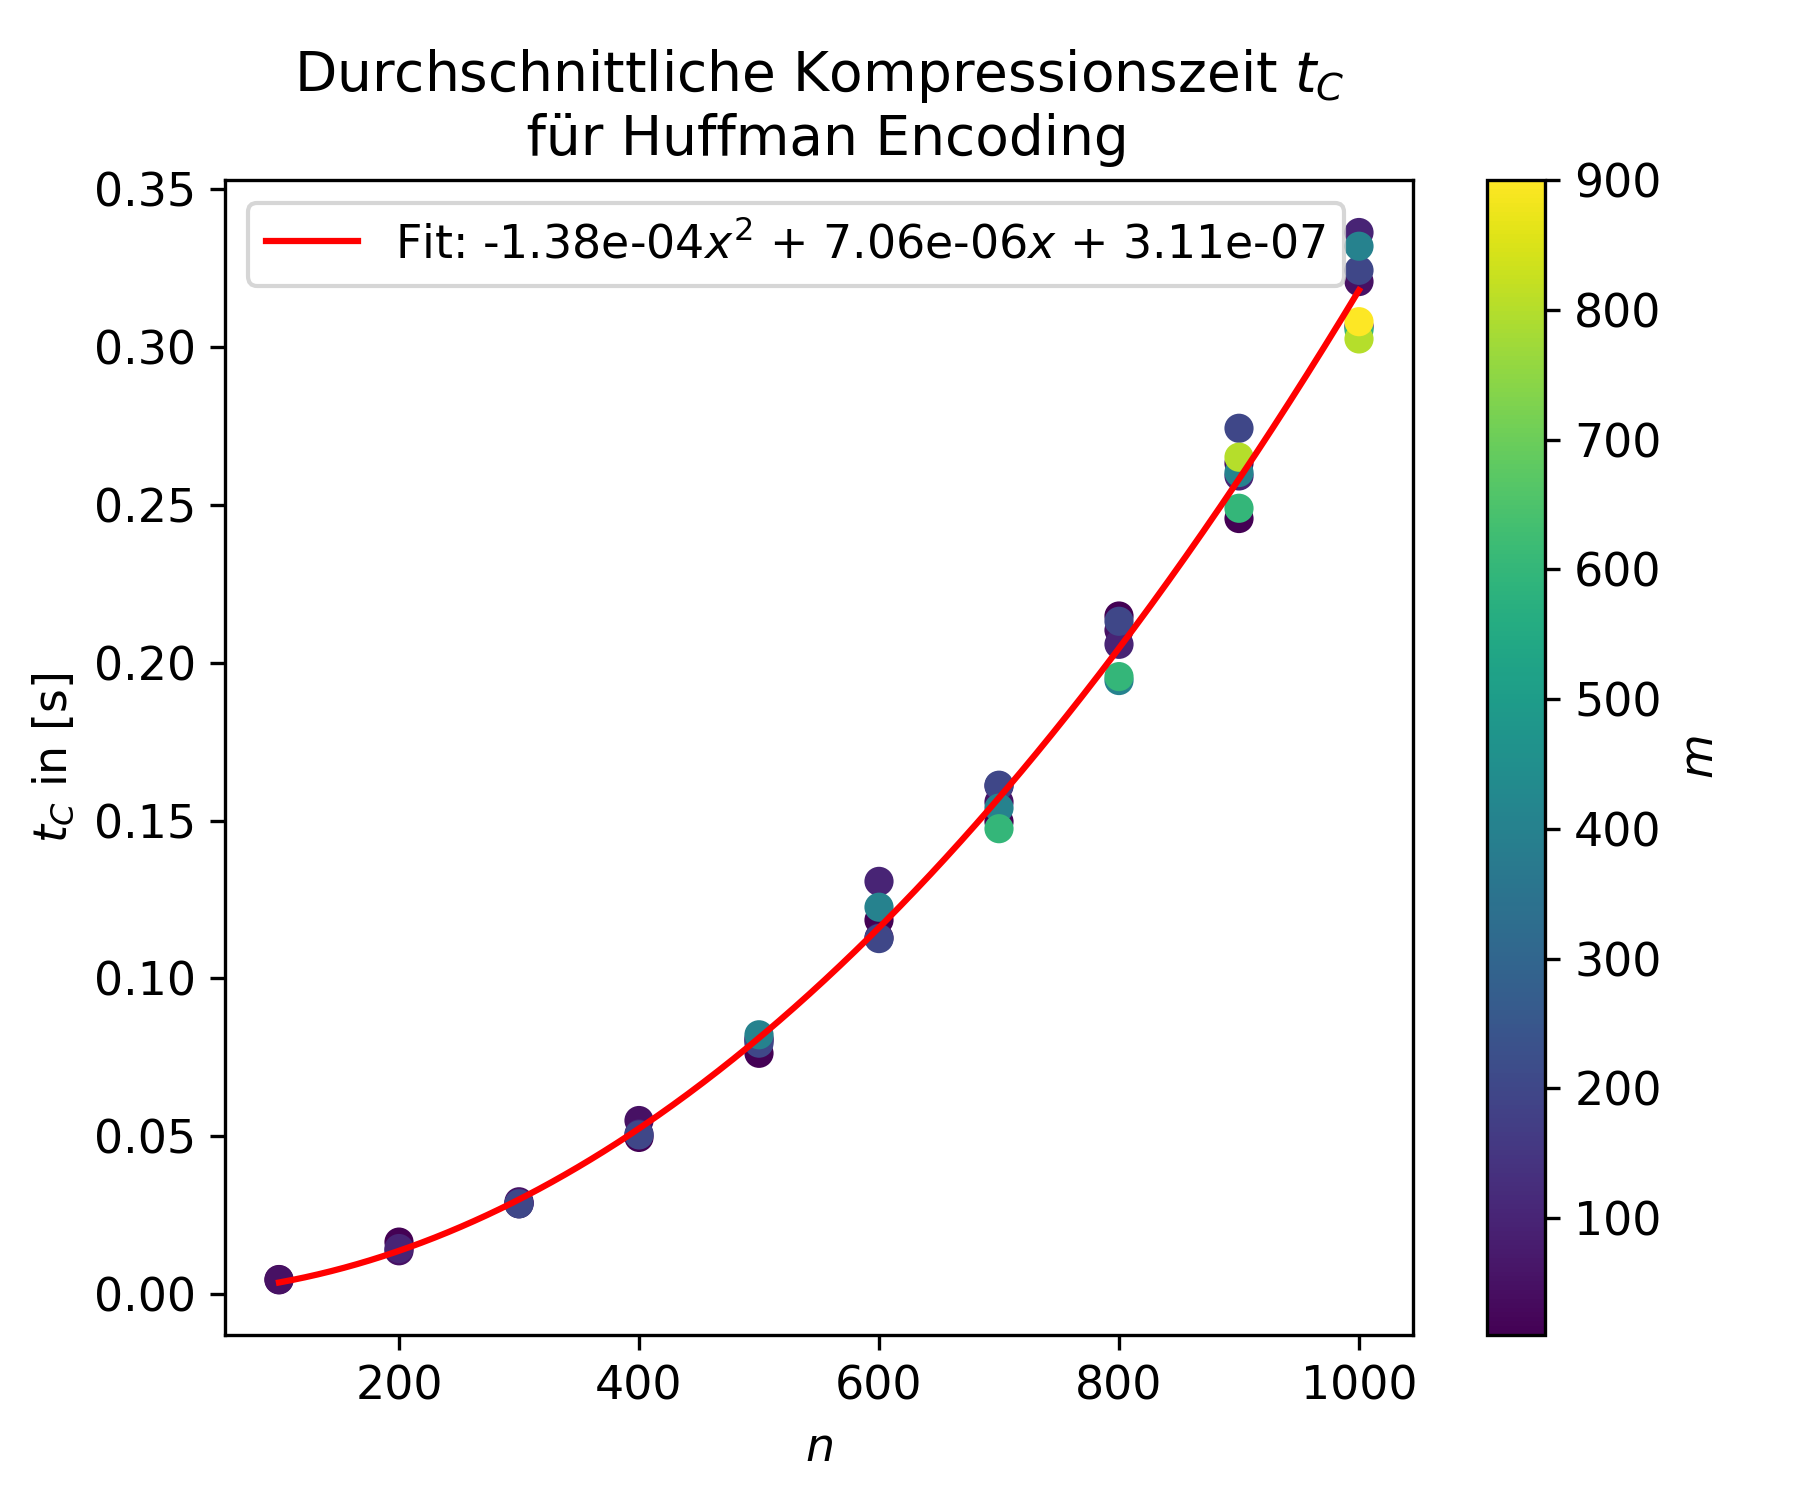
\includegraphics[width=0.7\textwidth]{images/huffmantime.png}
    \caption{Die gemessenen durchschnittlichen Kompressionszeiten für Huffman Encoding der Barábasi-Albert Graphen mit gegebenen Parametern $n$ (Anzahl Knoten und $m$ (Anzahl mit einem Knoten verbundene Kanten)}
    \label{fig:huffmantime}
\end{figure}

\subsection{Kompressionsfaktor}
\label{ch:compress_c_h}
Zur Bestimmung des Kompressionsfaktors $C$ wurden sämtliche Graphen aus dem Datensatz (vgl. Kapitel \ref{ch:datensatz} mittels Huffman Encoding komprimiert. 

\begin{table}[h!]
\centering
\begin{tabular}{@{}lr@{}}
\toprule
Variable    & Korrelationskoeffizient \\
\midrule
$n$ &        -0.240 \\
$m$ &        -0.193 \\
$d$ &        -0.675 \\
$E$ &         0.261 \\
\bottomrule
\end{tabular}
\caption{Korrelationskoeffizienten zwischen dem Kompressionsfaktor (Huffman Encoding) $C_{\text{Huffman}}$ und den Graph-Parametern $(n,m)$, der Graphdichte $d$ und der Anzahl Kanten $E$}
\label{tab:coefficients2}
\end{table}
Die Korrelation mit den beiden Graph-Parametern $n$ und $m$ ist klein, deshalb wurden zusätzlich die aus den Graphen ermittelten Grössen $E$ und $d$ untersucht. Die grösste (absolute) Korrelation mit dem Kompressionsfaktor $C_{\text{Huffman}}$ weist gemäss Tabelle \ref{tab:coefficients2} die Graph-Dichte $d$ auf, diese Korrelation ist negativ. 
Deshalb wird in Abbildung \ref{fig:chuffman} diese Abhängigkeit dargestellt.
Der Kompressionsfaktor $C$ ist für eine Dichte von ca. $0.4$ und Werte von $m<200$ maximal, nimmt mit Werten von $m>200$ stark ab.
\begin{figure}[h!]
    \centering
    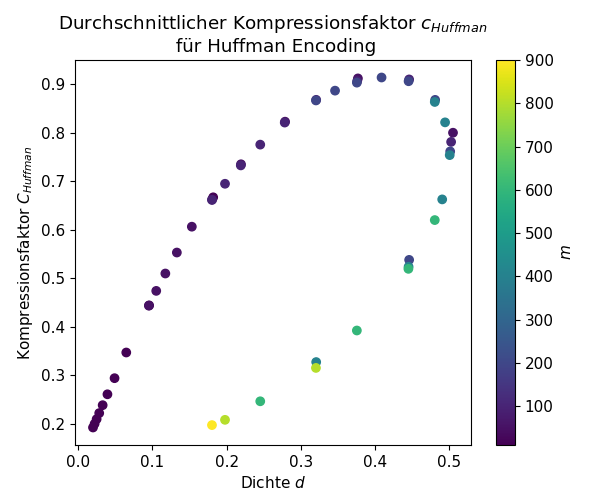
\includegraphics[width=0.7\textwidth]{images/avg_huffman_compression_density_no_outliers_color.png}
    \caption{Die gemessenen durchschnittlichen Kompressionsfaktoren für Huffman Encoding der Barábasi-Albert Graphen in Abhängigkeit der Dichte $d$ und des Graph-Parameters $m$}
    \label{fig:chuffman}
\end{figure}

\section{Kompression mittels $k^{2}$-Tree}
Die Kompression mittels $k^{2}$-Tree (vgl. \ref{ch:tree}) wurde analog zur Kompression mittels Huffman Encoding durchgeführt. Für sämtliche Messungen wurde der Parameter $k=2$ verwendet.
\subsection{Kompressionszeit}
Auch die Messungen zur Bestimmung der Kompressionszeit mittels $k^2$-Tree wurden auf dem gesamten Datensatz durchgeführt. Ebenfalls wurden die jeweils 10 Messungen pro Parameterpaar $(n,m)$ gemittelt, um den Einfluss von Varianzen abzuschwächen. Die Tabelle \ref{tab:coefficientstree} zeigt, dass die Kompressionszeit $t_{C}$ primär von der Anzahl Kanten $n$ im Graphen abhängt.
\begin{table}[h]
\centering
\begin{tabular}{@{}lr@{}}
\toprule
Variable    & Korrelationskoeffizient \\
\midrule
$n$ & 0.759 \\
$m$ & 0.187 \\
\bottomrule
\end{tabular}
\caption{Korrelationskoeffizienten zwischen der Kompressionszeit ($k^{2}$-Tree) und den Graph-Parametern $(n,m)$}
\label{tab:coefficientstree}
\end{table}

\begin{figure}[H]
    \centering
    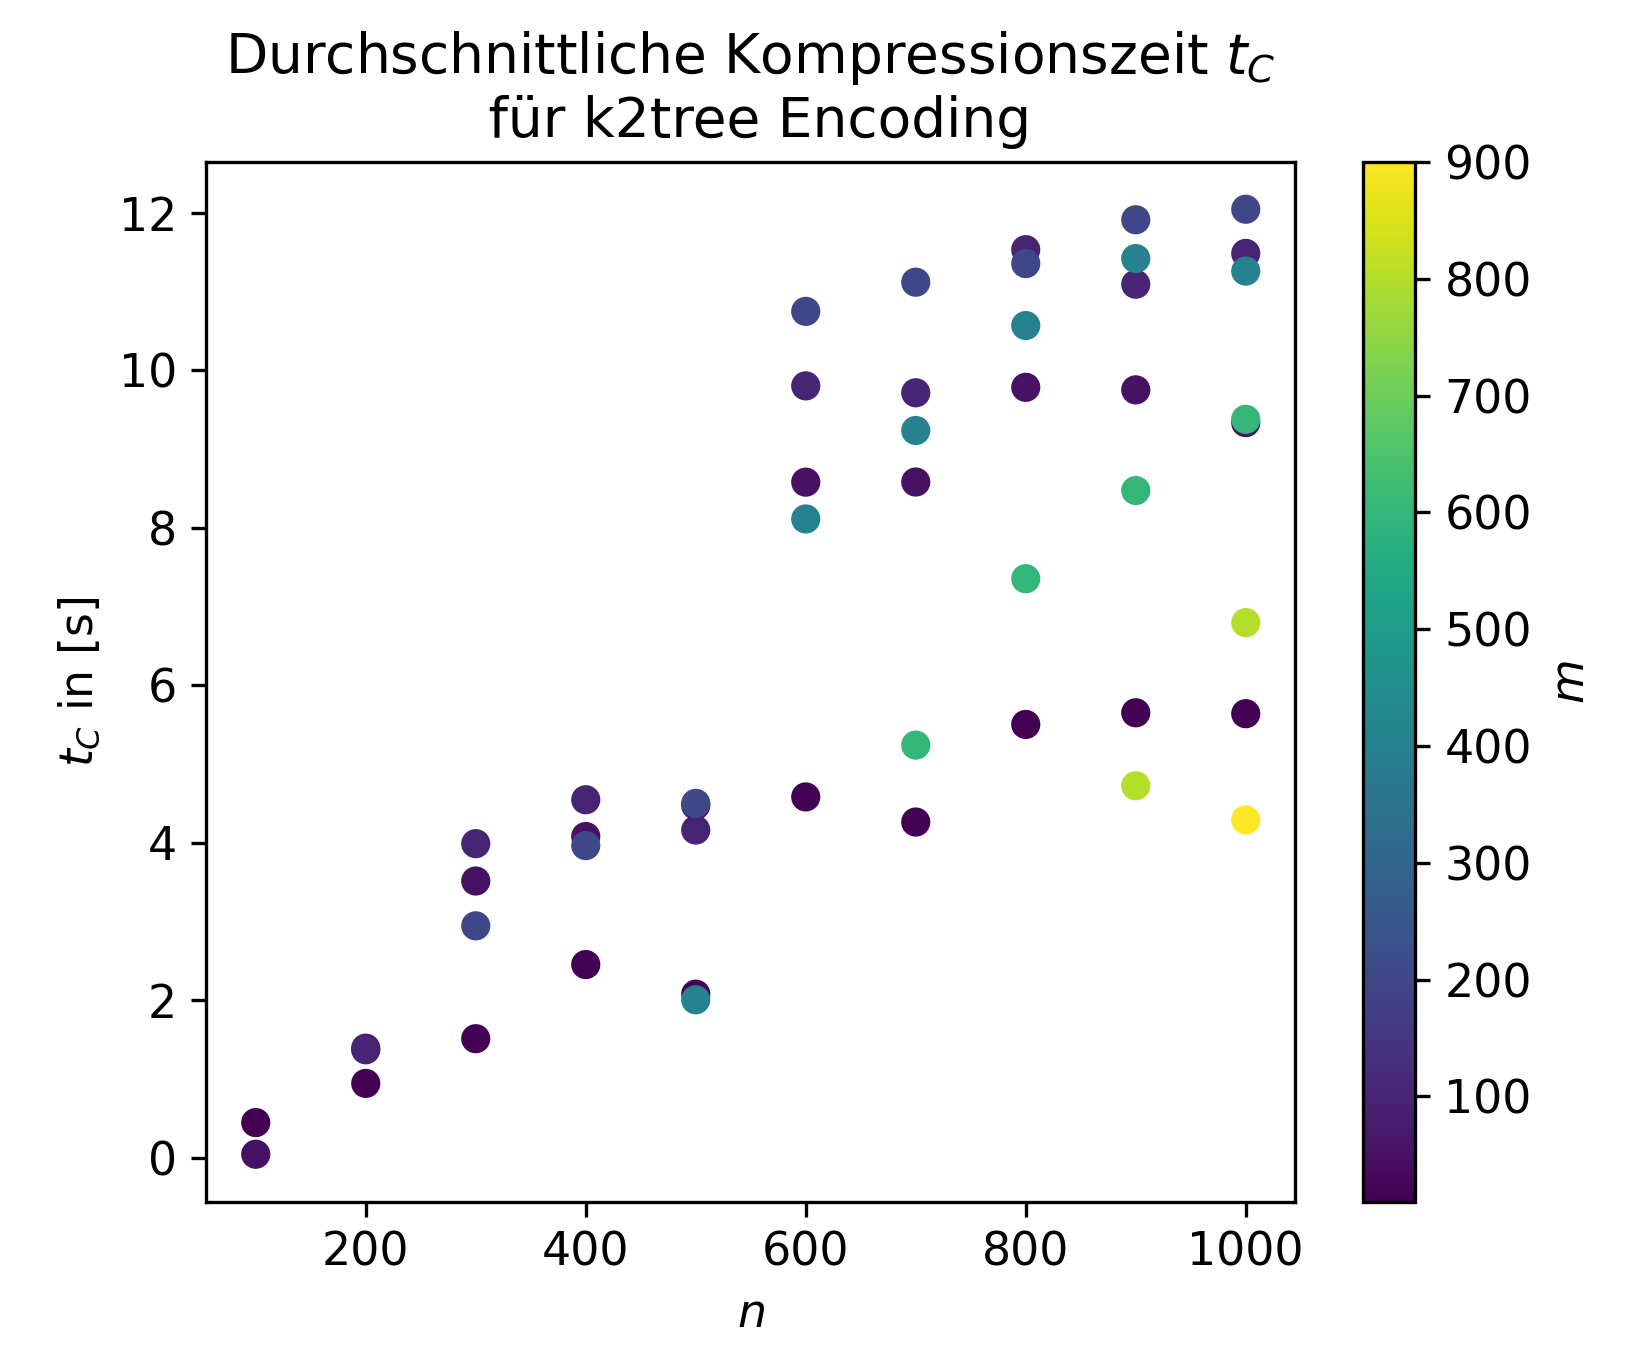
\includegraphics[width=0.7\textwidth]{images/average_k2tree_time_2d_filtered.png}
    \caption{Die bei der Kompression mittels $k^{2}$-Tree gemessenen Kompressionszeiten $t_{C}$ in Abhängigkeit der Anzahl Knoten $d$}
    \label{fig:compression_time_k2}
\end{figure}

\subsection{Kompressionsfaktor}
Der Kompressionsfaktor $C_{k2-Tree}$ für $k^{2}$-Tree wurde auf dem gesamten Datensatz gemessen, die jeweils 10 Messungen mit identischen Graph-Parametern $(n,m)$ wurden gemittelt. Auch hier wurden die Korrelationskoeffizienten der Graph-Parameter und der Graph-Eigenschaften $d$ und $E$ mit der Kompressionszeit bestimmt (vgl. Tabelle \ref{tab:coefficientstree2}).

\begin{table}[h]
\centering
\begin{tabular}{@{}lr@{}}
\toprule
Variable    & Korrelationskoeffizient \\
\midrule
$n$ & -0.455 \\
$m$ & -0.303 \\
\bottomrule
\end{tabular}
\caption{Korrelationskoeffizienten zwischen dem Kompressionsfaktor $C_{k2-Tree}$ und den Graph-Parametern $(n,m)$}
\label{tab:coefficientstree2}
\end{table}

\begin{figure}[H]
    \centering
    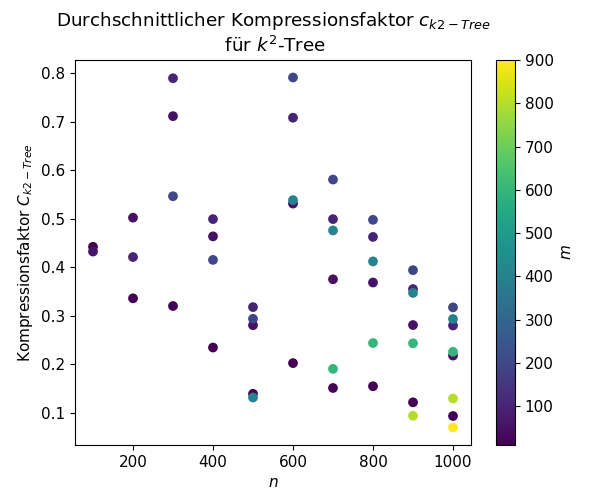
\includegraphics[width=0.7\textwidth]{images/avg_k2tree_compression_n_value_no_outliers_color.png}
    \caption{Der Kompressionsfaktor $C_{k2-Tree}$ in Abhängigkeit des Graph-Parameters $n$ (Anzahl Knoten) für die Kompression mittels $k^2$-Tree}
    \label{fig:compression_factor-k2}
\end{figure}

Analog zur Auswertung in Kapitel \ref{ch:compress_c_h} wird in Abbildung \ref{fig:compression_factor-k2_2} der Kompressionsfaktor $C_{k2-Tree}$ in Abhängigkeit der Dichte $d$ gezeigt. Insgesamt ist der Kompressionsfaktor sehr variabel, steigt mit steigender Dichte jedoch leicht an.

\begin{figure}[H]
    \centering
    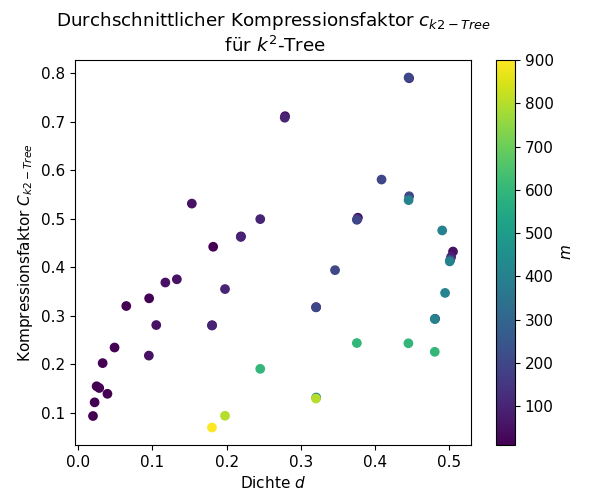
\includegraphics[width=0.7\textwidth]{images/avg_k2tree_compression_density_no_outliers_color.png}
    \caption{Der Kompressionsfaktor $C_{k2-Tree}$ in Abhängigkeit der Graphdichte $d$ für die Kompression mittels $k^2$-Tree}
    \label{fig:compression_factor-k2_2}
\end{figure}

\chapter{Diskussion} % Diskutieren Sie Ihre Ergebnisse im Kontext der Forschungsfrage und der vorhandenen Literatur. Identifizieren Sie Stärken und Schwächen Ihrer Studie.
Die im Rahmen dieser Arbeit durchgeführten Messungen zeigen für beide verwendeten Kompressionsalgorithmen Stärken und Schwächen bezüglich der untersuchten Messgrössen Kompressionsfaktor und Kompressionszeit. 

\section{Kompressionsfaktor}
Der Kompressionsfaktor hängt bei der Verwendung von Huffman Encoding von der Dichte $d$ des Graphen ab und erreicht für die untersuchten Graphen bei einer Dichte von ungefähr 0.4 das Maximum. Der Kompressionsfaktor, welcher durch die Verwendung von $k^2$-Tree erreicht wird, liegt für den gesamten Messbereich unter den durch Huffman maximal erreichbaren Werte (vgl. Abbildung \ref{fig:compression_factor-vergleich}). 
\begin{figure}[H]
    \centering
    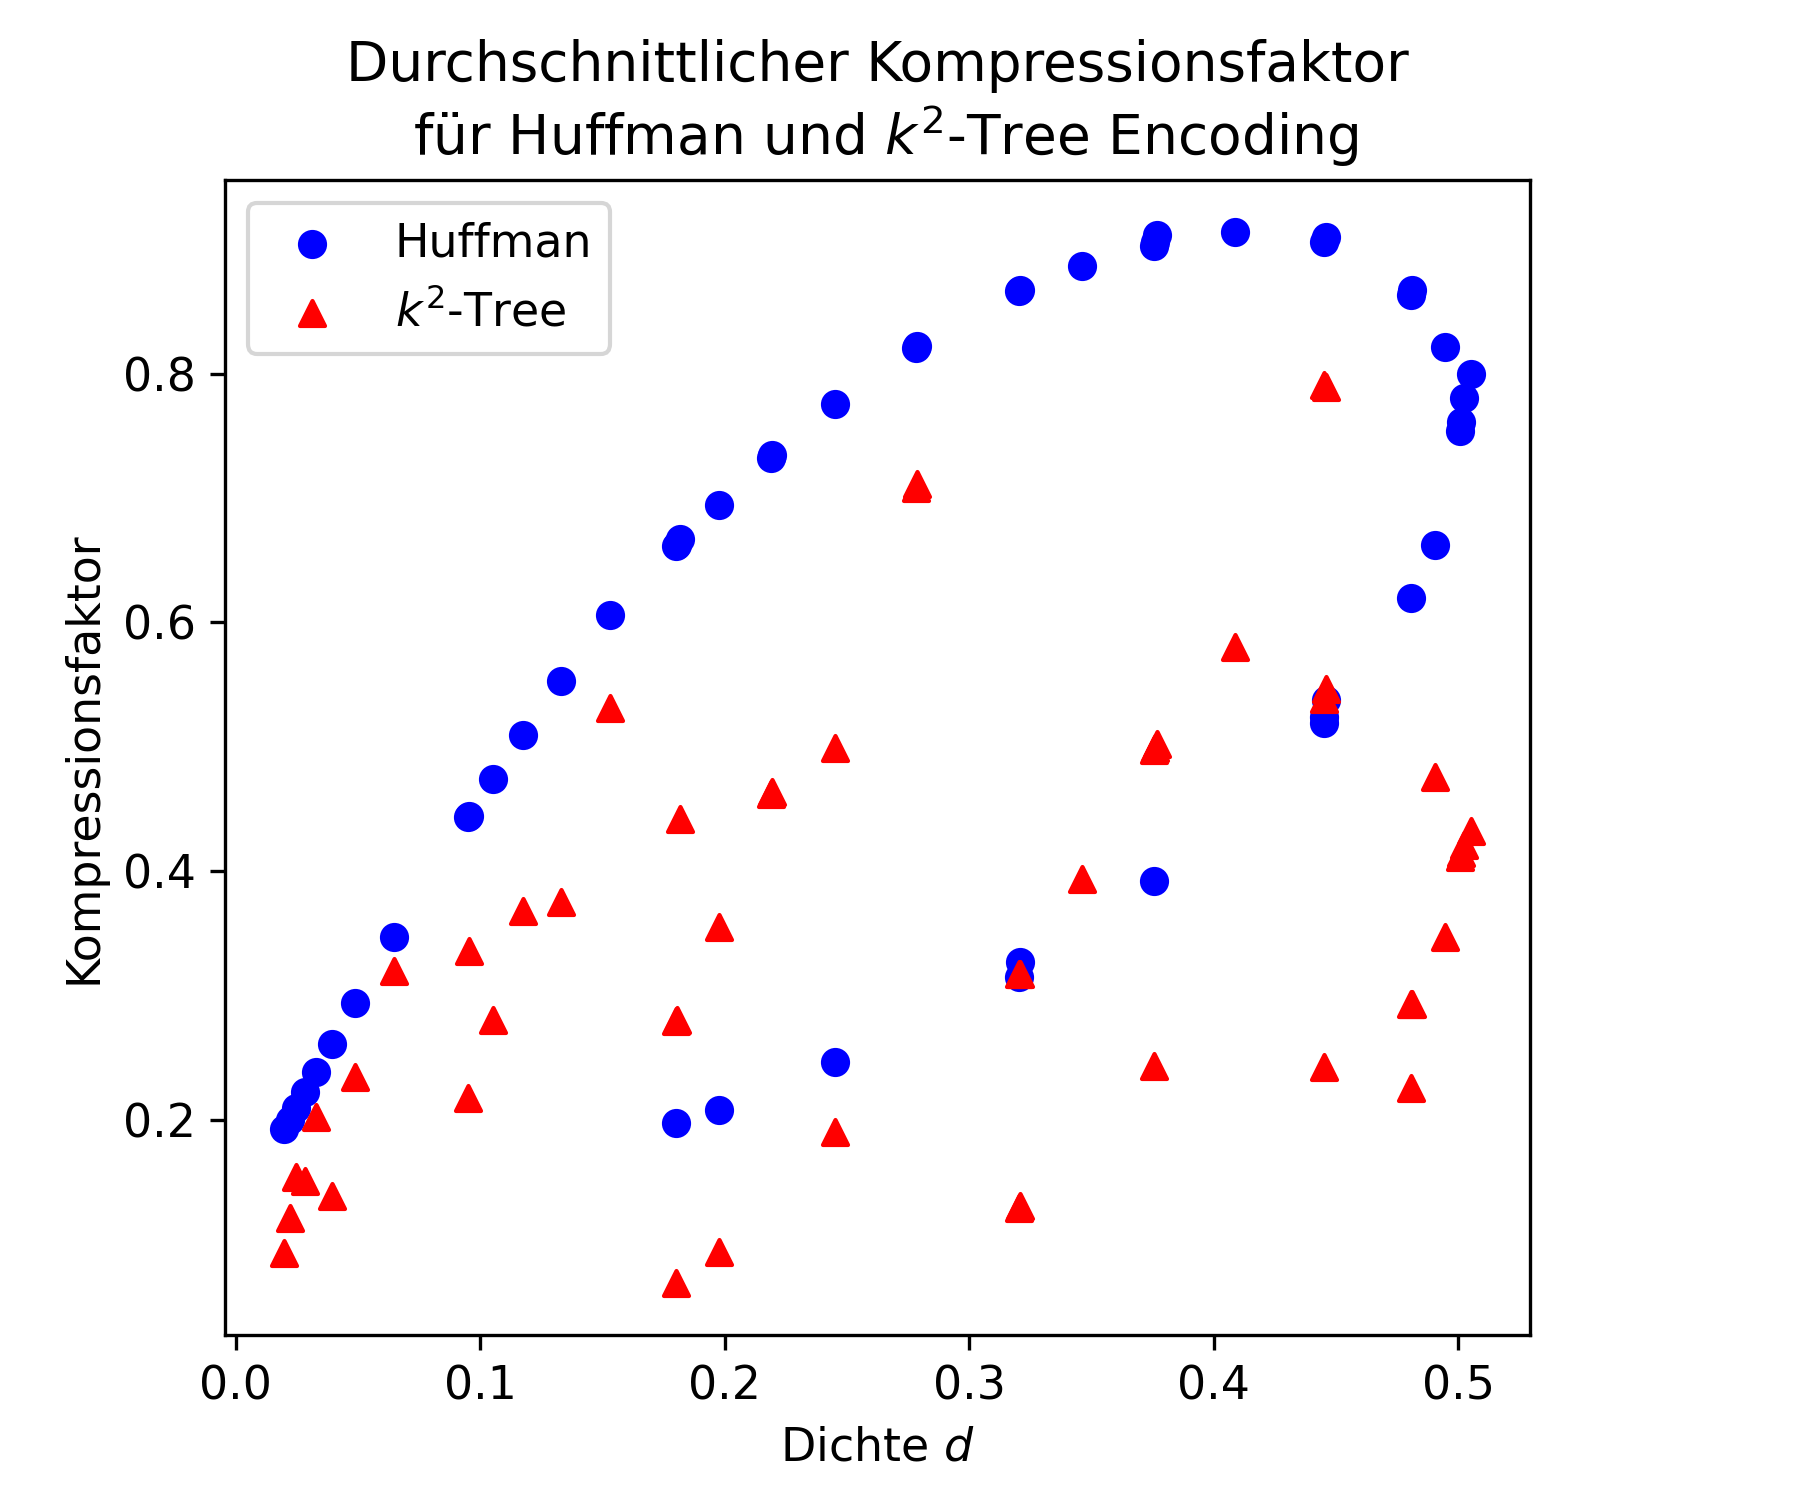
\includegraphics[width=0.7\textwidth]{images/avg_compression_density_no_outliers_color.png}
    \caption{Vergleich der erreichten Kompressionsfaktoren für die beiden untersuchten Algorithmen Huffman Encoding und $k^2$-Tree}
    \label{fig:compression_factor-vergleich}
\end{figure}
Die Abhängigkeit des Kompressionsfaktors von der Dichte beim Einsatz von Huffman Encoding und dessen Maximum bei einer Dichte von $0.4$ hängt vermutlich von der Entropie der Kantenliste ab, welche für die Graphen gemäss Gleichung \ref{eq:entropy} auf Seite \pageref{eq:entropy} ein Minimum besitzen muss. Diese Vermutung müsste in einer weiterführenden Arbeit untersucht werden.

\section{Kompressionszeit}
Die Daten zeigen eine hohe Korrelation zwischen der Anzahl der Knoten $n$ in den untersuchten Graphen und der Zeit $t_{\text{Huffman}}$, die Huffman Encoding für die Kompression benötigt. Die Abhängigkeit der Kompressionszeit von der Anzahl Knoten lässt sich für die untersuchten Barábasi-Albert Graphen mit einer quadratischen Funktion darstellen.
\begin{figure}[H]
    \centering
    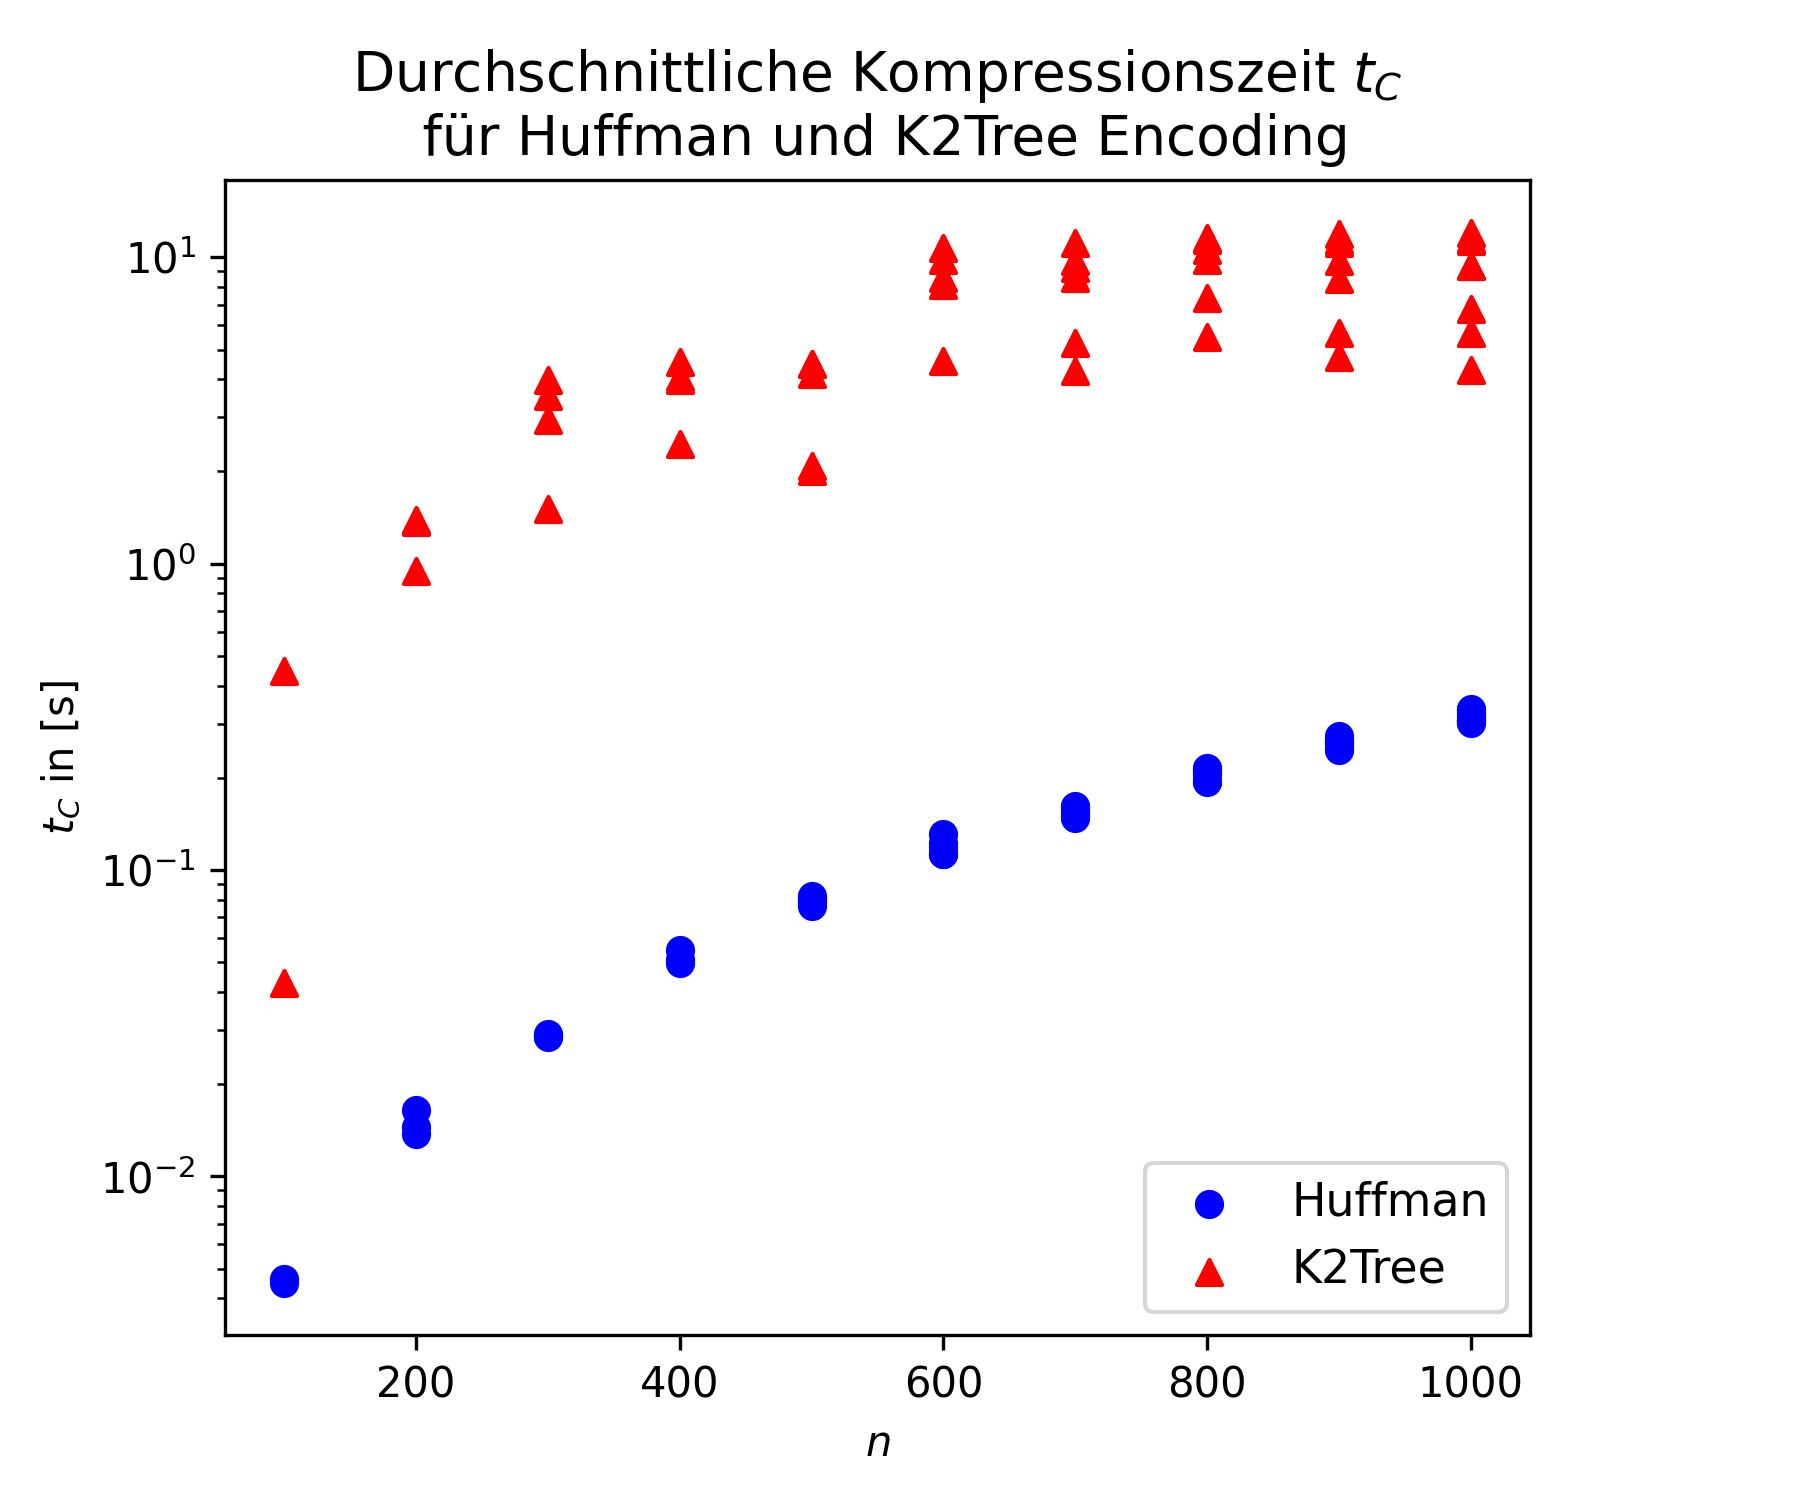
\includegraphics[width=0.7\textwidth]{images/average_time_2d_filtered_comparison_same_plot.png}
    \caption{Vergleich der Kompressionszeiten für die beiden untersuchten Algorithmen Huffman Encoding und $k^2$-Tree}
    \label{fig:compression_time-vergleich}
\end{figure}
 Huffman Encoding ist also bezüglich der Kompressionszeit weniger effizient für grössere Graphen. Im Gegensatz dazu hängt $k^2$-Tree etwas weniger stark von der Grösse der Graphen ab, die Kompressionszeit steigt jedoch in der Tendenz mit $n$ an, was auch in der relativ hohen Korrelation von $0.759$ zur Kompressionszeit sichtbar wird. Der direkte Vergleich zwischen den beiden Algorithmen (vgl. Abbildung \ref{fig:compression_time-vergleich}) zeigt, dass die Kompressionsfaktoren von Huffman Encoding auf den untersuchten Graphen durch $k^2$-Tree nicht erreicht werden. 


\chapter{Schlussfolgerungen} % Fassen Sie Ihre Hauptergebnisse zusammen und beantworten Sie Ihre Forschungsfrage. Diskutieren Sie die Auswirkungen Ihrer Forschung und schlagen Sie Bereiche für zukünftige Forschungen vor.
Die in dieser Arbeit gestellten Forschungsfragen (vgl. Kapitel \ref{ch:problemstellung}) konnten anhand der durchgeführten Untersuchungen wie folgt beantwortet werden:
\begin{enumerate}
    \item Die Effektivität der beiden Kompressionsalgorithmen Huffman Encoding und $k^2$-Tree in Bezug auf Kompressionsfaktor und -Zeit bei der Kompression von Barábasi-Albert Graphen hängt stark von den spezifischen Eigenschaften des Graphen ab. In Bezug auf den Kompressionsfaktor erreicht Huffman Encoding bei einer Dichte von ca. 0.4 das Maximum. Der durch $k^2$-Tree erreichte Kompressionsfaktor bleibt über alle untersuchten Graphen unter den Maximalwerten von Huffman Encoding. Die Kompressionszeit von Huffman Encoding steigt mit dem Quadrat der Anzahl Knoten an, bleibt jedoch über den gesamten Messbereich bis $n=1000$ stark unter den durch $k^2$-Tree benötigten Kompressionszeiten. 
    \item Die Leistung der beiden Algorithmen unterscheiden sich stark. Beide hängen bezüglich der Kompressionszeit von der Grösse der Graphen ab, wobei die Abhängigkeit bei Huffman Encoding stärker ausgeprägt ist. Die Dichte hat einen grossen Einfluss auf den Kompressionsfaktor. 
    \item Die Leistung von Huffman Encoding hängt stark von Dichte und Grösse der Graphen ab. Huffman Encoding eignet sich bei den untersuchten Graphen bei einer Dichte um den Maximalwert von $0.4$. Weitere Untersuchungen mit grösseren Graphen müssten zeigen, ob sich die Leistung von $k^2$-Tree bei noch grösseren Graphen mit kleinerer Dichte verbessern würde.
\end{enumerate}
Zusammenfassend lässt sich sagen, dass von den beiden Algorithmen nur Huffman Encoding wirklich gut zur Kompression von Barábasi-Albert Graphen geeignet ist. $k^2$-Tree kann im untersuchten Bereich seine Stärke durch seine Abhängigkeit von leeren Bereichen in der Adjazenzmatrix bei zufällig erzeugten, skalenfreien Graphen nicht ausspielen. 
\chapter{Zukünftige Arbeiten} % Sprechen Sie über die Möglichkeiten, wie diese Arbeit in der Zukunft fortgesetzt oder erweitert werden könnte.
Die in dieser Arbeit durchgeführten Untersuchungen haben Erkenntnisse zur Leistungsfähigkeit von Huffman Encoding und $k^2$-Tree bei der Kompression von Barábasi-Albert-Graphen geliefert. Die gewonnenen Erkenntnisse werfen aber gleichzeitig neue Fragen auf, welche in zukünftigen Forscungsarbeiten untersucht werden können:
\begin{itemize}
    \item Eventuell könnte sich $k^2$-Tree bei noch grösseren und weniger dichten Barábasi-Albert Graphen als etwas effizienter herausstellen, eine weitere Untersuchung könnte zeigen, in welchem Bereich das Optimum für $k^2$-Tree liegen könnte.
    \item Für die Kompression von Barábasi-Albert Graphen müssten zwingend weitere Algorithmen untersucht werden, welche auf die speziellen Eigenschaften dieser Graphen optimiert sind.
    \item In der Arbeit wurde nicht untersucht, wie gut sich die unterschiedlichen Kompressionsarten für Analysen der Graphen oder Operationen auf den Graphen eignen. Diese Aspekte sind jedoch bei der Beurteilung eines Kompressionsalgorithmus zentral.
\end{itemize}
Die vorliegenden Forschungsergebnisse bilden eine Grundlage für zukünftige Untersuchungen in diesem Bereich. Die gewonnenen Erkenntnisse können dazu verwendet werden,  Algorithmen zur Kompression von Barábasi-Albert Graphen zu optimieren.

\bibliographystyle{plain}
\bibliography{bibtexfile.bib}
% oder besser
% \bibliography{myBibTeXFile.bib}
\appendix
\chapter{Code}
\section{Code zum Generieren der Graphen}
\label{code:graphgen}
\begin{minted}[breaklines=true, breakanywhere]{python}
def generate_graphs():
    graph_list = []
    adj_list = []
    nm_list = []
    n_values = [100,200,300,400,500,600,700,800,900,1000]
    m_values = [10,50,100,200,400,600,800,900,1000]
    
    # Create directory for saving graphs
    if not os.path.exists('Graphs'):
        os.makedirs('Graphs')

    for n in n_values:
        for m in m_values:
            if m < n:
                for i in range(10):  # Repeat 10 times for each combination of n and m
                    graph = nx.barabasi_albert_graph(n, m)
                    adj = nx.adjacency_matrix(graph).todense().tolist()
                    graph_list.append(graph)
                    adj_list.append(adj)
                    nm_list.append((n, m))  # Save n, m used for generating this graph

                    # Save graph
                    nx.write_graphml(graph, f'Graphs/graph_{n}_{m}_{i}.graphml')
    return graph_list, adj_list, nm_list
\end{minted}

\section{Code Messung Kompressionszeiten}
\label{code:compression_time}
\begin{minted}[breaklines=true, breakanywhere]{python}
def compare_algorithms(graph_list, adj_list, nm_list):
    results = []
    
    for (graph, adj, nm) in zip(graph_list, adj_list, nm_list):
        n_nodes = graph.number_of_nodes()
        m_edges = graph.number_of_edges()
        density = nx.density(graph)
        n_value, m_value = nm  # n, m used for generating this graph
        
        # Measure time for k2tree compression
        start_time = time.time()
        k2_tree = k2t.k2_tree(adj, 2)
        k2tree_time = time.time() - start_time
        k2tree_compression = k2t.count_nodes(k2_tree)/(n_nodes**2)  # correct here

        # Measure time for Huffman compression
        adj_bin = ''.join(str(e) for row in adj for e in row)
        start_time = time.time()
        huffman_compress = huff.compress_binary_data(adj_bin)
        huffman_time = time.time() - start_time
        huffman_compress = len(huffman_compress)/(n_nodes**2)  # correct here

        results.append((n_value, m_value, n_nodes, m_edges, density, k2tree_time, k2tree_compression, huffman_time, huffman_compress))
    
    return results
\end{minted}

\section{Code Implementierung Huffman Encoding}
\label{code:huffman}
\begin{minted}[breaklines=true, breakanywhere]{python}
from collections import defaultdict
import heapq

class Node:
    def __init__(self, symbol, frequency, left=None, right=None):
        self.symbol = symbol
        self.frequency = frequency
        self.left = left
        self.right = right

    def __lt__(self, other):
        return self.frequency < other.frequency

def calculate_frequency(data):
    frequency = defaultdict(int)
    for i in range(len(data) - 7):
        pattern = data[i:i+8]
        frequency[pattern] += 1
    return frequency

def build_huffman_tree(frequency):
    heap = []
    for pattern, freq in frequency.items():
        heapq.heappush(heap, Node(pattern, freq))

    while len(heap) > 1:
        node1 = heapq.heappop(heap)
        node2 = heapq.heappop(heap)
        merged = Node(None, node1.frequency + node2.frequency, node1, node2)
        heapq.heappush(heap, merged)

    return heap[0]

def assign_codes(node, code='', codes={}):
    if node.symbol:
        codes[node.symbol] = code
    else:
        assign_codes(node.left, code + '0', codes)
        assign_codes(node.right, code + '1', codes)

    return codes

def encode_data(data, codes):
    encoded_data = ''
    i = 0
    while i < len(data) - 7:
        pattern = data[i:i+8]
        if pattern in codes:
            encoded_data += codes[pattern]
            i += 8
        else:
            encoded_data += pattern
            i += 1
    return encoded_data

def compress_binary_data(data):
    frequency = calculate_frequency(data)
    huffman_tree = build_huffman_tree(frequency)
    codes = assign_codes(huffman_tree)
    encoded_data = encode_data(data, codes)
    return encoded_data
\end{minted}
\section{Code Implementierung K2-Tree}
\label{code:k2tree}
\begin{minted}[breaklines=true, breakanywhere]{python}
import numpy as np

# Node class for k2-tree
class Node:
    def __init__(self, value):
        self.value = value
        self.children = []

    # used for printing the tree
    def __repr__(self, level=0):
        ret = "\t" * level + repr(self.value) + "\n"
        for child in self.children:
            ret += child.__repr__(level+1)
        return ret

# Generate a k2-tree from the adjacency matrix
def k2_tree(matrix, k):
    n = len(matrix)

    matrix_array = np.array(matrix)
    if np.all(matrix_array == 0):
        return Node(0)

    if n == 1:
        return Node(matrix_array[0, 0])

    nodes = []
    size = n // k
    for i in range(k):
        for j in range(k):
            nodes.append(k2_tree(matrix_array[i*size:(i+1)*size, j*size:(j+1)*size].tolist(), k))

    node = Node(any(node.value == 1 for node in nodes))
    node.children = nodes

    return node

def count_nodes(node):
    return 1 + sum(count_nodes(child) for child in node.children)
\end{minted}

\end{document}


